% Setting up the document class and essential packages
\documentclass[12pt, a4paper]{article} % Increased font size
\usepackage[utf8]{inputenc}
\usepackage{geometry}
\geometry{a4paper, margin=1in}
\usepackage{graphicx} % For including figures
\usepackage{array}    % For better table formatting
\usepackage{booktabs} % For professional-looking tables
\usepackage{enumitem} % For customizing lists
\usepackage{titlesec} % For customizing section headings
\usepackage{parskip}  % For paragraph spacing
\usepackage{amsmath, amssymb} % For math symbols
\usepackage{setspace} % For line spacing
\usepackage[T1]{fontenc}
\usepackage{times} % Using Times font for professionalism

\onehalfspacing % Set line spacing to 1.5

% Starting the document
\begin{document}

% Creating the title page
\title{\LARGE\textbf{Issues and Challenges of Software Projects in Environmental Systems}} % Made title larger and bold
\author{
Mahnoor Akter Esha \\ Roll: 22201087 \\
Tanjina Akter Nisa \\ Roll: 22201086 \\
Md. Daudul Islam \\ Roll: 22201088}
\date{June 2025}
\maketitle

\begin{center}
\textbf{A Project Proposal Submitted in Partial Fulfillment of the Requirements for the Degree of Bachelor of Science in Computer Science and Engineering} \\
\vspace{0.5em}
University of Asia Pacific \\
Department of Computer Science and Engineering \\
\vspace{0.5em}
\textbf{Supervised by:} \\
Dr. Subhra Prosun Paul \\
Assistant Professor \\
Department of Computer Science and Engineering \\
University of Asia Pacific
\end{center}

% Certificate page (Page 2)
\clearpage
\section*{Certificate}
This is to certify that the thesis proposal titled ``\textit{Issues and Challenges of Software Projects in Environmental Systems}'' is the original work of Tanjina Akter Nisa, Mahnoor Akter Esha, and Md. Daudul Islam, carried out under the supervision of Dr. Subhra Prosun Paul. The work was conducted in the Department of Computer Science and Engineering at the University of Asia Pacific. This proposal is submitted in partial fulfillment of the requirements for the Bachelor of Science in Computer Science and Engineering degree.

\vspace{3em}
Chairman of the Committee (Supervisor) \\
\rule{0.5\textwidth}{0.4pt} \\
Dr. Subhra Prosun Paul \\
Assistant Professor \\
Department of Computer Science and Engineering \\
University of Asia Pacific (UAP)

\vspace{3em}
Head of the Department \\
\rule{0.5\textwidth}{0.4pt} \\
Dr. Shah Murtaza Rashid Al Masud \\
Professor \\
Department of Computer Science and Engineering \\
University of Asia Pacific (UAP)

% Acknowledgements page (Page 3)
\clearpage
\section*{Acknowledgements}
We express our heartfelt gratitude to our supervisor, Dr. Subhra Prosun Paul, Assistant Professor, for his invaluable guidance, insightful feedback, and unwavering support throughout the development of this thesis proposal. His expertise and encouragement were instrumental in shaping this work.

We extend our appreciation to the faculty members of the Department of Computer Science and Engineering at the University of Asia Pacific for their academic support and constructive suggestions. We are also grateful to our classmates for their collaboration and encouragement.

Finally, we acknowledge the researchers and scholars whose published works provided critical insights and a foundation for this proposal. Their contributions enriched our understanding of the challenges in environmental software systems.

% Table of Contents (Page 4)
\clearpage
\section*{Abstract}
Environmental software projects are essential for tackling global challenges related to climate change, resource management, and ecosystem monitoring. These projects typically involve technologies such as sensors, satellites, and drones to collect data for analysis—data that informs scientists and policymakers about critical environmental issues. However, developing such software poses significant difficulties. These include equipment malfunctions in extreme conditions, inconsistent integration of various tools, a shortage of skilled labor, and high costs with long-term returns. Hardware may fail in deserts or oceans, and the software must manage large-scale, complex data. Finding experts who are proficient in both environmental science and technology is particularly challenging.

Moreover, environmental systems often require high precision and real-time data processing, which imposes strict requirements on software architecture. Development is further complicated by heterogeneous data sources, system scalability, and security concerns. This paper highlights these challenges—especially those related to scalability—and proposes strategies to enhance performance. The aim is to improve the efficiency, reliability, and real-world impact of environmental software systems.

\textbf{Keywords:} Environmental software, software engineering challenges, hardware challenges, software integration, manpower expertise, cost-benefit analysis, sustainable development, real-time processing.

\section{Introduction}
The world today faces serious environmental challenges. Climate change is causing global temperatures to rise, air and water pollution are endangering human health, and natural resources such as clean water and forests are being depleted rapidly. In this context, environmental software plays a crucial role. These software systems are designed to collect and analyze environmental data. For instance, specialized sensors can monitor urban air quality or track river water levels. Such data enables scientists, governments, and environmental organizations to make informed decisions for protecting ecosystems.

\subsection*{1.1 Role of Environmental Software}
With increasing challenges like climate change, deforestation, and rapid urban expansion, environmental software has become more important than ever. These tools are widely used for monitoring air and water quality, protecting endangered species, and forecasting natural disasters such as floods or cyclones [\cite{ref1}. Countries such as Bangladesh, India, and Indonesia are already implementing sensor-based platforms to collect real-time data on rainfall, river levels, and pollution. This real-time data supports faster, more accurate decision-making. However, despite their promise, many of these projects struggle to meet expectations due to persistent challenges.

\subsection*{1.2 Challenges in Environmental Software Projects}
Several factors contribute to the difficulties faced by these projects. Environmental projects are typically interdisciplinary, involving professionals from fields such as ecology, geology, civil engineering, and computer science. These experts often use different terminologies and methodologies, and poor communication among them can lead to unclear project goals, incorrect budgeting, and mismatched technical choices.

A major technical challenge is managing the enormous volume and complexity of environmental data, which comes from diverse sources such as satellites, drones, and ground-based sensors. This data is often inconsistent, incomplete, or in incompatible formats. Software must be capable of cleaning, processing, and analyzing this data in real-time. Tools like Artificial Intelligence (AI) and Machine Learning (ML) are useful for predicting environmental risks \cite{ref3}, yet many systems lack the infrastructure or technical capacity to implement these solutions effectively \cite{ref4}.

\subsection*{1.3 Hardware and Connectivity Limitations}
Many environmental software systems are deployed in remote or harsh environments, such as mountainous regions, forests, or river basins, where electricity and internet connectivity are unreliable. The hardware used must therefore be durable and energy-efficient. For example, in Bangladesh, the Flood Forecasting and Warning Centre (FFWC) uses river and rainfall data to predict floods. Yet the system sometimes fails to deliver accurate and timely warnings due to limitations in satellite data, computing resources, and trained personnel \cite{ref6}.

\subsection*{1.4 Project Management and Cost Issues}
These challenges are not purely technical. Many environmental software projects lack long-term planning. They may start with enthusiasm but fail due to inadequate budgeting, weak management, or lack of trained personnel \cite{ref7}. Additionally, the benefits of such projects—like improved air quality or reduced pollution—often take time to materialize, which makes it harder to secure funding or sustained support. Consequently, many promising projects are abandoned mid-way.

There is a strong need for low-cost, scalable, and easy-to-maintain solutions tailored to the specific needs of the local environment. Imported technologies may not be suitable for regions such as Bangladesh or India, and local customization is critical.

\begin{figure}[h]
    \centering
    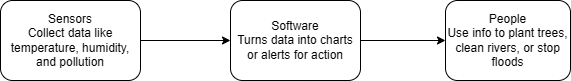
\includegraphics[width=1.0\textwidth]{figure1}
    \caption{How Environmental Software Works}
    \label{fig:how_software_works}
\end{figure}

\begin{figure}[h]
    \centering
    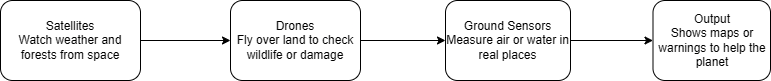
\includegraphics[width=1.0\textwidth]{figure2}
    \caption{Sources of Environmental Data}
    \label{fig:data_sources}
\end{figure}

\section{Background Study}
Historically, environmental data was recorded manually, such as writing down rainfall or temperature. Today, technologies like satellites, drones, and smart sensors allow for rapid and precise data collection. These tools are used to forecast floods, monitor pollution, and track wildlife. Modern infrastructure such as cloud computing supports the storage and analysis of large datasets, while AI helps predict events like storms and wildfires.

Despite these advancements, challenges remain. Hardware can fail in harsh environments. Software struggles with managing massive, disorganized datasets. The shortage of skilled personnel further increases operational costs. While some organizations establish data-sharing policies, compliance is inconsistent. Additionally, software systems must evolve continuously to keep up with rapid technological change.

\begin{table}[h]
\centering
\begin{tabular}{|p{3cm}|p{5cm}|p{5cm}|}
\hline
\textbf{Tool} & \textbf{Functionality} & \textbf{Challenge} \\
\hline
Sensors & Measure environmental parameters (e.g., air, water, soil quality) & Prone to failure in extreme conditions \\
\hline
Drones & Capture aerial imagery and videos for monitoring & Difficult to repair in remote regions \\
\hline
Cloud Computing & Store and process large-scale environmental data & Requires reliable and high-speed internet \\
\hline
Artificial Intelligence (AI) & Predict trends and environmental risks (e.g., floods, fires) & Demands significant computational resources and expertise \\
\hline
\end{tabular}
\vspace{0.5em}
\caption{Tools Used in Environmental Software}
\end{table}

\section{Analysis: Main Issues}

\subsection{Hardware Issues}
Environmental hardware such as sensors and drones often operates in harsh environments like deserts, forests, or oceans. Devices can fail due to exposure to rain, extreme temperatures, or humidity. Many remote regions lack electricity, necessitating the use of batteries or solar panels, which can be unreliable. Furthermore, hardware components from different manufacturers may not be compatible, causing integration challenges.

\subsection{Software Issues}
Environmental software must aggregate data from satellites, drones, and ground sensors, often in varying formats. This makes data integration complex. Some programs may crash or slow down, especially during emergencies that require quick decision-making. Additionally, these systems face cybersecurity risks, making data protection a high priority.

\subsection{Manpower Problems}
Professionals with expertise in both environmental science and technology are rare. Training such individuals requires time and resources. Communication barriers may arise between scientists and engineers due to disciplinary differences, delaying project progress.

\subsection{Cost and Benefit Challenges}
Environmental software development is costly. Equipment, specialized software, and skilled personnel all contribute to high expenses. However, the benefits—such as improved public health or reduced environmental damage—are often long-term. This delay in visible outcomes makes it harder to secure funding or maintain stakeholder interest, resulting in many projects being discontinued prematurely.

\section{Recommendations}

\subsection{Addressing Hardware Issues}
\begin{itemize}
    \item Use durable, weather-resistant equipment designed for outdoor deployment.
    \item Install backup power solutions, such as solar panels and batteries, to ensure uninterrupted operation.
    \item Design interoperable hardware systems to enable smooth integration across platforms.
\end{itemize}

\subsection{Addressing Software Issues}
\begin{itemize}
    \item Adopt modular software design to simplify updates and troubleshooting.
    \item Standardize data formats to facilitate seamless data exchange and analysis.
    \item Conduct regular testing and implement strong cybersecurity protocols.
\end{itemize}

\subsection{Addressing Manpower Issues}
\begin{itemize}
    \item Offer training programs to upskill team members in both environmental science and software development.
    \item Enhance collaboration through communication tools and regular meetings.
    \item Partner with educational institutions and online platforms to recruit and train emerging talent.
\end{itemize}

\subsection{Addressing Cost Challenges}
\begin{itemize}
    \item Launch pilot projects to validate ideas before scaling up.
    \item Leverage open-source software to reduce licensing costs.
    \item Seek funding from government grants or collaborate with eco-conscious corporations.
\end{itemize}

\section{Conclusion and Future Work}
Environmental software offers significant potential for addressing pressing global issues such as climate change, pollution, and resource degradation. These systems enable data-driven decisions that can safeguard natural ecosystems. Nevertheless, several barriers—technical, organizational, and financial—still hinder their effectiveness. Hardware reliability, software scalability, manpower availability, and project funding remain key concerns. 

Future work should focus on developing adaptive, low-cost, and scalable solutions tailored to regional needs. Collaborations between technologists and environmental scientists must be strengthened to build systems that are both technically sound and environmentally meaningful.

% References section

\section{References}

\begin{thebibliography}{9}

\bibitem{ref1}
Wei, Yunxiao, Chao Han, and Zuolong Yu. ``An environment safety monitoring system for agricultural production based on artificial intelligence, cloud computing and big data networks.'' \textit{Journal of Cloud Computing} 12, no. 1 (2023): 83.

\bibitem{ref2}
Chen, Siguang, Jiasheng Zhou, Xiaoyao Zheng, and Xiukai Ruan. ``Energy-efficient data collection scheme for environmental quality management in buildings.'' \textit{IEEE Access} 6 (2018): 57324-57333.

\bibitem{ref3}
Weersink, Alfons, Evan Fraser, David Pannell, Emily Duncan, and Sarah Rotz. ``Opportunities and challenges for big data in agricultural and environmental analysis.'' \textit{Annual Review of Resource Economics} 10, no. 1 (2018): 19-37.

\bibitem{ref4}
Singh, Sooryansh, Avinash Kumar, Apurv Prasad, and Nitish Bharadwaj. ``IoT based water quality monitoring system.'' Proceedings of the IRFIC (2016).

\bibitem{ref5}
Fenton, Norman E., and Niclas Ohlsson. ``Quantitative analysis of faults and failures in a complex software system.'' \textit{IEEE Transactions on Software Engineering} 26, no. 8 (2002): 797-814.

\bibitem{ref6}
Felländer, Anna, Jonathan Rebane, Stefan Larsson, Mattias Wiggberg, and Fredrik Heintz. ``Achieving a data-driven risk assessment methodology for ethical AI.'' \textit{Digital Society} 1, no. 2 (2022): 13.

\bibitem{ref7}
Komeil, Raisian, Yahaya Jamaiah, and Deraman Aziz. ``Current challenges and conceptual model of green and sustainable software engineering.'' (2016).

\end{thebibliography}
\end{document}
